% 6.3：依据表3、表4及同源的已保存数值场分析结果；图6使用用户提供的两张PNG。
\subsection{结果分析}
\label{sec:p2-analysis}

表\ref{tab:p2T}、表\ref{tab:p2C}及图\ref{fig:p2-evolution}展示前$3\ \mathrm{h}$的温湿变化，
图中药材曲线分别对应中心、$r=1\ \mathrm{cm}$处及表面，与表格采用同一数值解。

\subsubsection{温度逐渐趋于均匀}

图\ref{fig:p2-evolution}(a)显示，\textbf{表面先升温，中心响应滞后，随后各位置温度逐渐靠拢。}
表面与中心的温差由$0.5\ \mathrm{h}$时的$3.2238\tempunit$
缩小至$3\ \mathrm{h}$时的$0.1169\tempunit$，
此时表列各位置的温度为$49.8495$--$49.9664\tempunit$，已接近烘房温度。

\begin{figure}[!htbp]
\centering
% 保持原图6的0.98\textwidth宽度及264.543625/634.2825高宽比。
% 以相同范围裁去两张PNG的白边，完整保留标题、图例、单位及最右侧刻度。
% trim按源PNG的300 dpi换算；仅指定高度以保持原比例，轴框宽度及水平位置沿用原图。
\setlength{\unitlength}{0.98\textwidth}
\begin{picture}(1,0.417075396)
  \put(0.004323459,0.014316401){\makebox(0,0)[lb]{%
    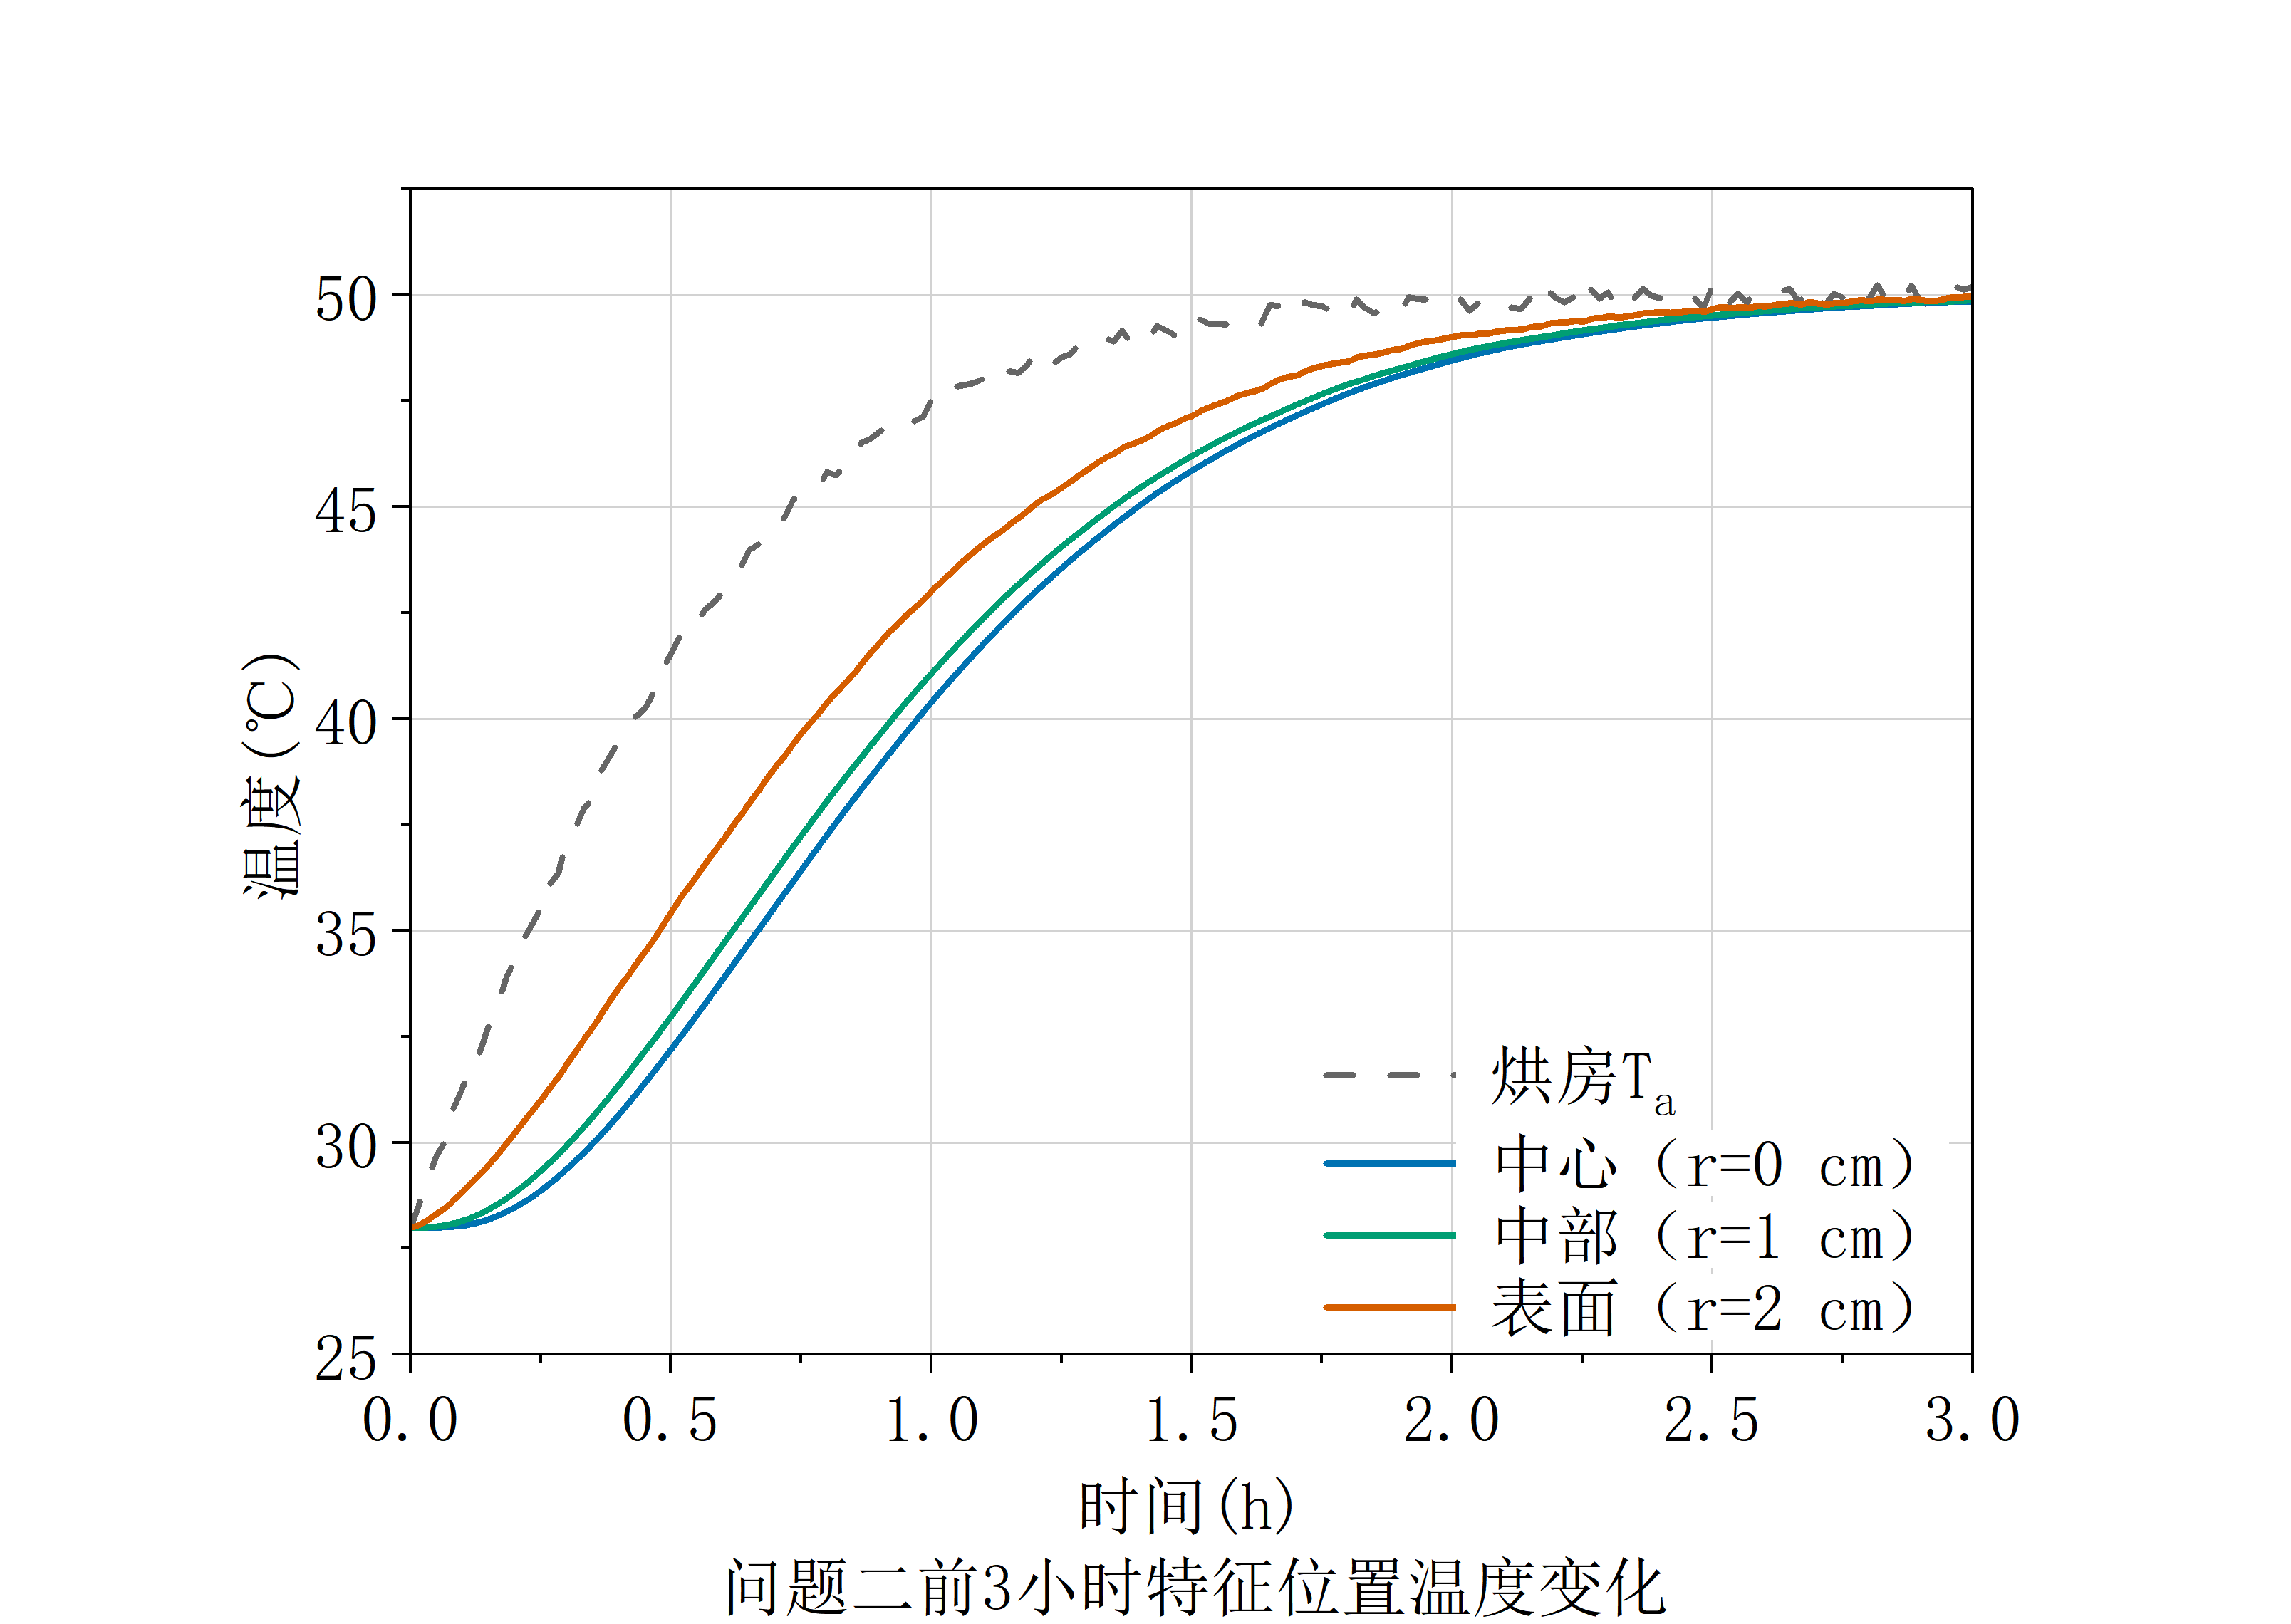
\includegraphics[trim={66.000bp 26.400bp 87.840bp 32.400bp},clip,
      height=0.385911668\unitlength]{图7(a).png}}}
  \put(0.503372671,0.014316401){\makebox(0,0)[lb]{%
    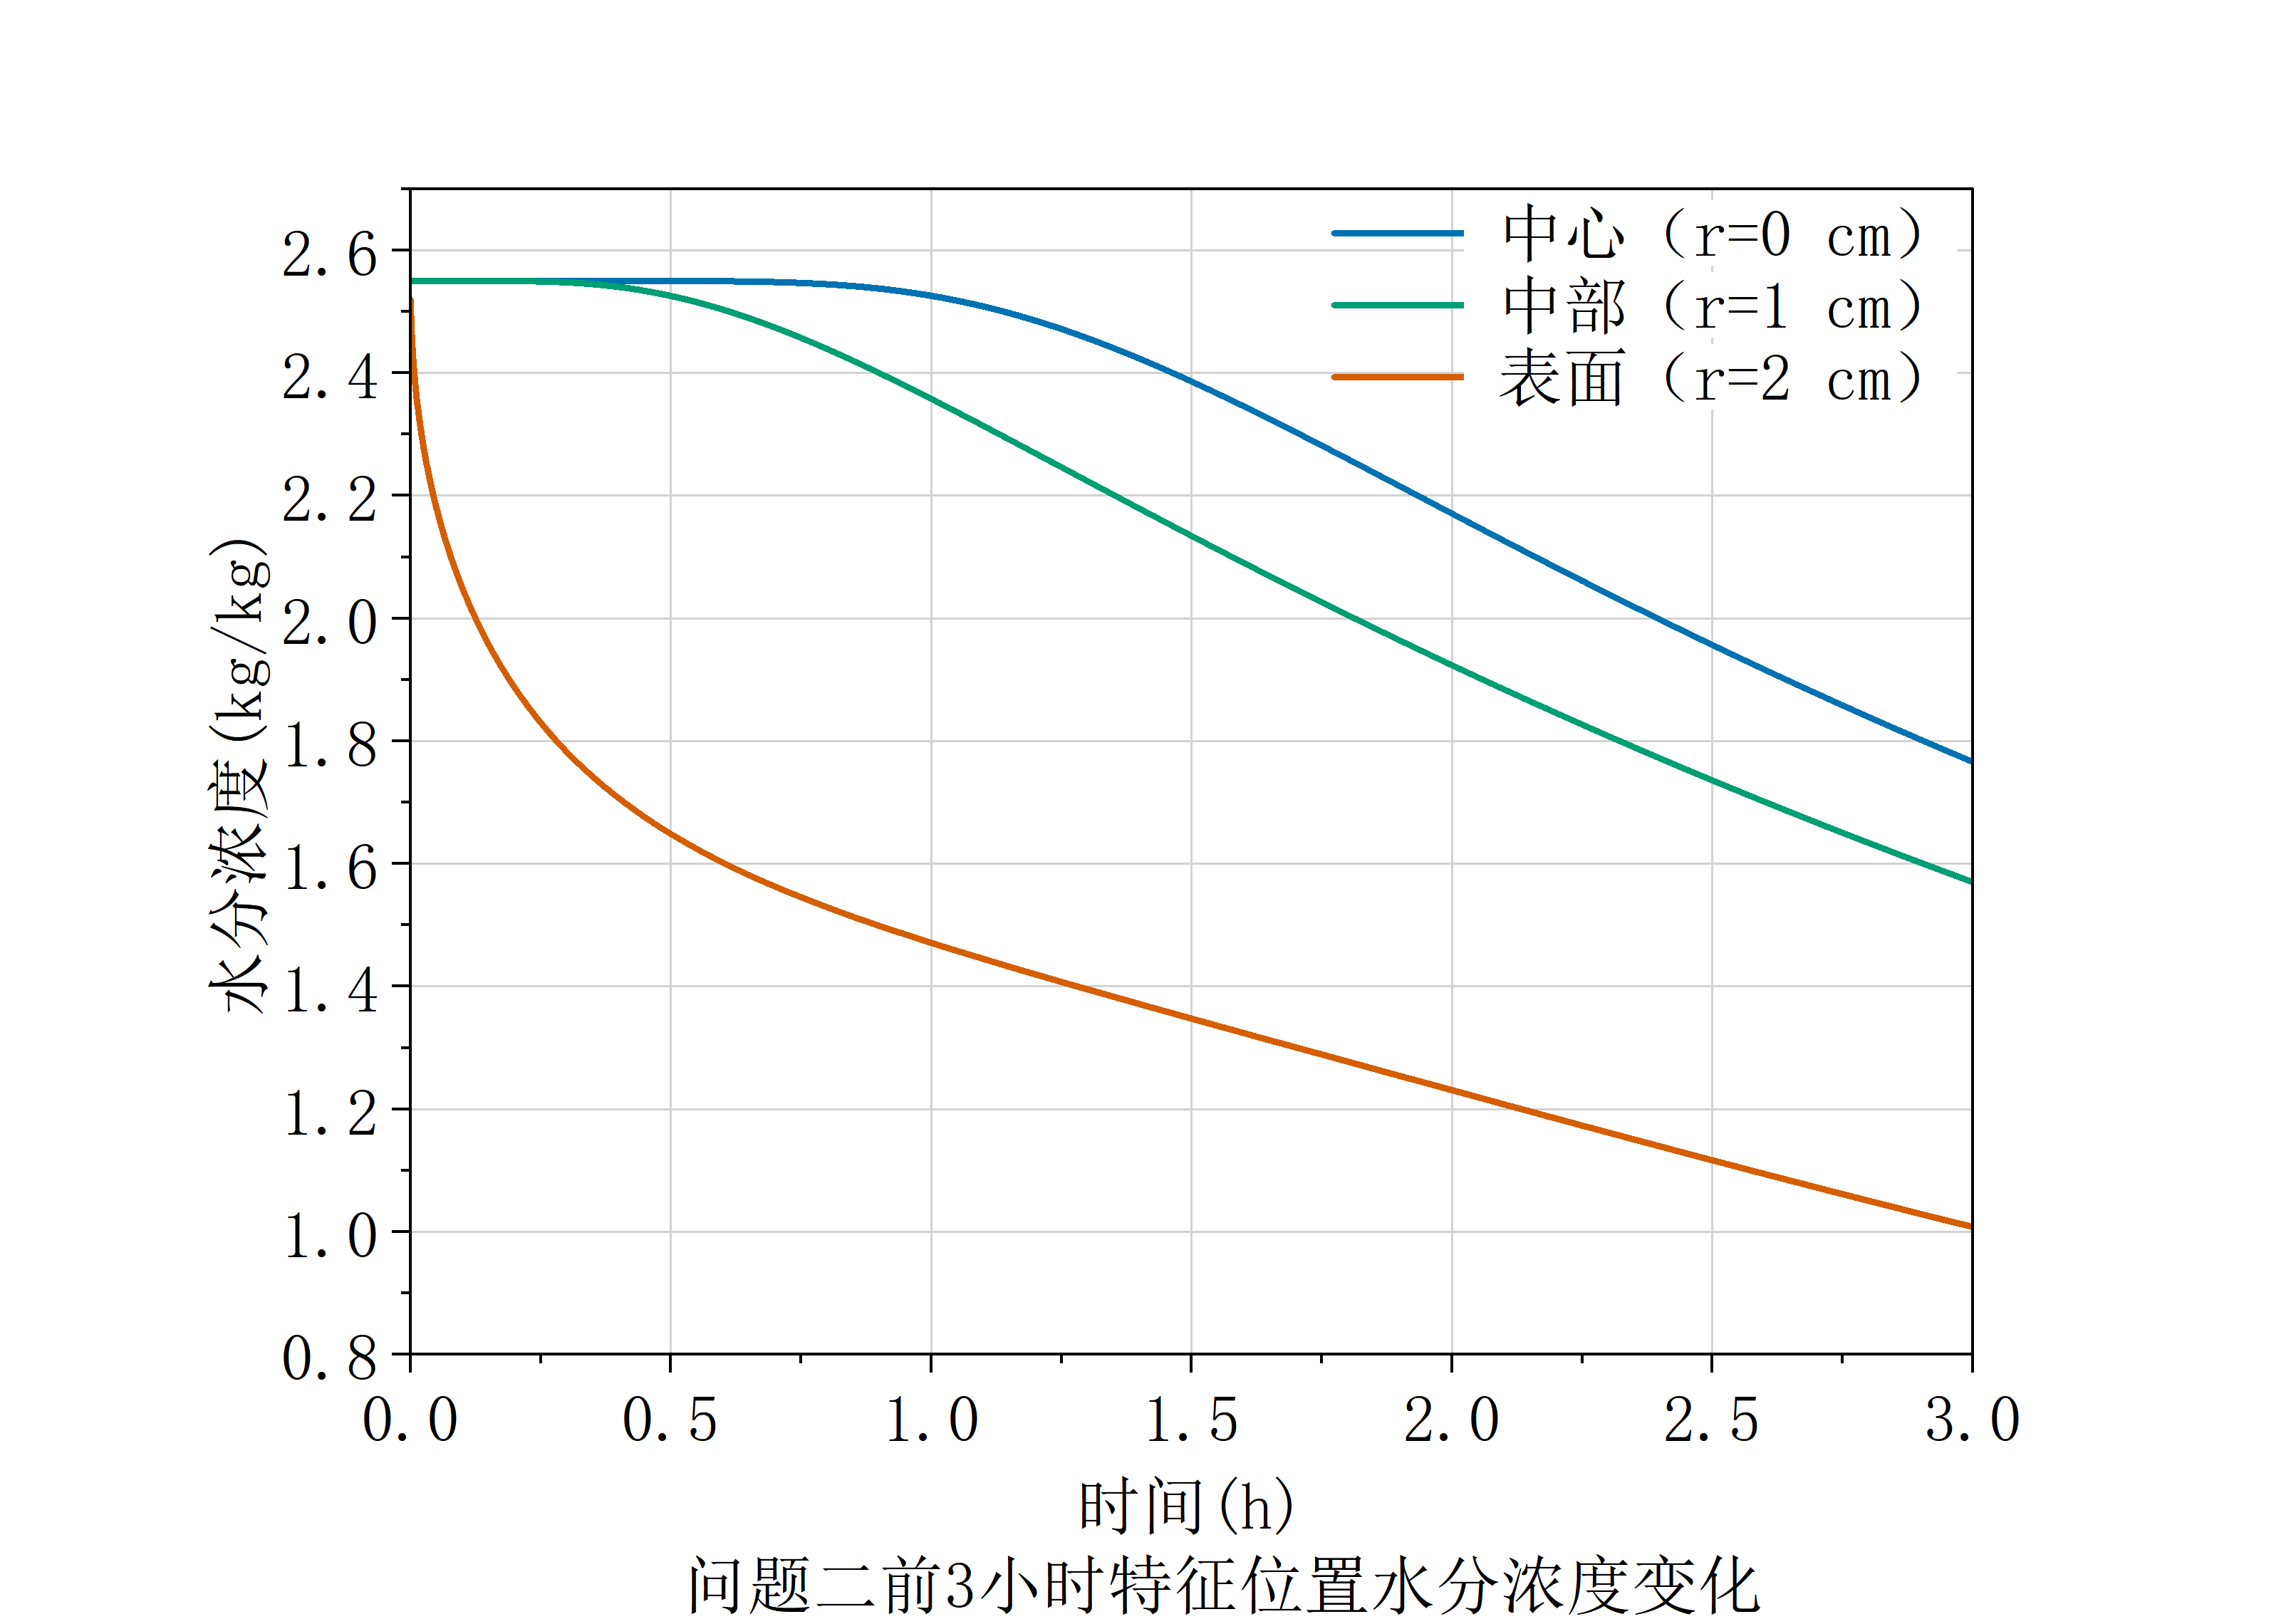
\includegraphics[trim={66.000bp 26.400bp 87.840bp 32.400bp},clip,
      height=0.385911668\unitlength]{图7(b).png}}}
\end{picture}
\caption{问题二前3 h特征位置的温度和含水率变化}
\label{fig:p2-evolution}
\end{figure}

\subsubsection{水分滞后与变物性作用}

图\ref{fig:p2-evolution}(b)显示，表面含水率初期迅速下降，中心随后才明显失水。
中心与表面的差值由$0.5\ \mathrm{h}$时的$0.9013\cunit$
增至$1\ \mathrm{h}$时的$1.0546\cunit$，
再降至$3\ \mathrm{h}$时的$0.7581\cunit$。
这一先增后减的变化反映了表面先失水、内部随后参与的过程，
但本时段末仍保留明显的内湿外干分布。

$3\ \mathrm{h}$时中心和表面含水率分别为$1.7662\cunit$、$1.0081\cunit$。
将对应温湿状态代入式\eqref{eq:p2-properties}，所得扩散系数约为
$1.24\times10^{-8}\ \mathrm{m^2/s}$和
$1.03\times10^{-8}\ \mathrm{m^2/s}$。
虽然表面温度略高，较干外层的扩散能力仍偏低，说明在这两个位置的比较中，
较低含水率的影响超过了微小温差对扩散的促进作用。
\textbf{因此，温度趋于均匀与水分脱除并不同步，局部含水率仍通过物性影响后续水分迁移。}
